\section{Pythagorean Theorem}
The Pathagrean Theorem is most commonly stated as
\[a^2 + b^2 = c^2\]
\\
Where a and b refer to the legs of a right triangle and c refers to the hypotenuse.\\
\\
\subsection{Derivation}
A square can be constructed of 4 right triangles as shown below.\\
\begin{center}
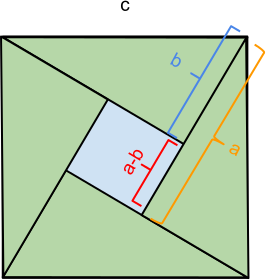
\includegraphics[width=8cm]{Trigonometry/pythagorus_diag1}
\end{center}
The area of the square, \(c^2\), is equal to the area of the 4 right triangles plus the area of the inner square.\\

\begin{align*}
c^2 =& 4\frac{ab}{2} + (a-b)^2\\
c^2 =& 2ab + a^2 -2ab + b^2 \\
c^2 =& a^2 + b^2
\end{align*}

\section{Sum and Difference of Sine}

\section{Sum and Difference of Cosine}

\section{Double Angle Identity for Sine}
The Double Angle Identity for sine is most commonly stated as
\[\sin{(2u)} = 2\sin{(u)}cos{(u)}\]

\subsection{Derivation}

\begin{center}
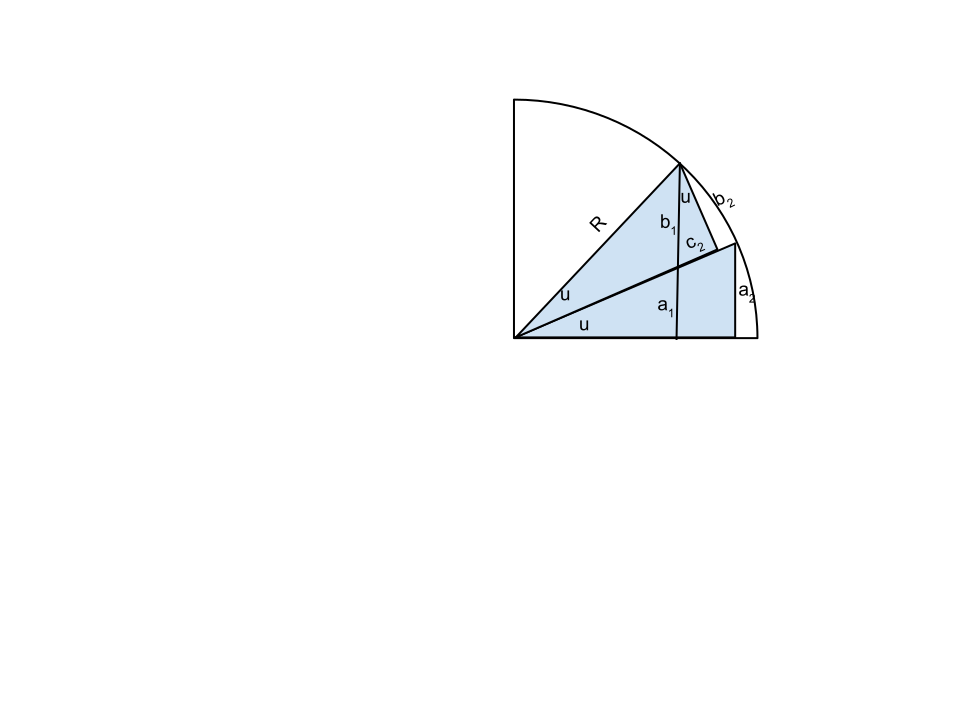
\includegraphics[width=8cm]{Trigonometry/Sine_double_angle}
\end{center}

With respect to the diagram above
\[R\sin{(2u)} = a_1 + b_1\]
Find \(a_1 \text{ and } b_1\)\\
\\
For \(a_1\) \\
\begin{align*}
a_1 &= c_2\sin{(u)} \\
c_1 + c_2 &= R\cos{(u)} \\
c_1 &= b_1\sin{(u)} \\
c_2 &=  R\cos{(u)} - b_1\sin{(u)} \\ 
a_1 &= (R\cos{(u)} - b_1\sin{(u)})\sin{(2u)}
\end{align*}
\\
For \(b_1\) \\
\begin{align*}
b_2 &= a_2 \\
b_1\cos{(u)} &= R\sin{(u)} \\
b_1 &= R\tan{(u)}
\end{align*}
\\
So
\begin{align*}
R\sin{(2u)} &= a_1 + b_1 \\
R\sin{(2u)} &= (R\cos{(u)} - b_1\sin{(u)})\sin{(u)} + b_1 \\
R\sin{(2u)} &= R\cos{(u)}\sin{(u)} -b_1\sin^2{(u)} +b_1 \\
R\sin{(2u)} &= R\cos{(u)}\sin{(u)} + b_1(1 -\sin^2{(u)})\\
R\sin{(2u)} &= R\cos{(u)}\sin{(u)} + b_1\cos^2{(u)} \\
R\sin{(2u)} &= R\cos{(u)}\sin{(u)} + R\tan{(u)}\cos^2{(u)} \\
sin{(2u)} &= \cos{(u)}\sin{(u)} + \sin{(u)}\cos{(u)} \\
sin{(2u)} &= 2\sin{(u)}\cos{(u)} 
\end{align*}
\\
Thus
\[sin{(2u)} = 2\sin{(u)}\cos{(u)} \]

\section{Double Angle Identity for Cosine}